%! TEX TS-program = LuaLaTeX

% Gemini theme
% See: https://rev.cs.uchicago.edu/k4rtik/gemini-uccs
% A fork of https://github.com/anishathalye/gemini

\documentclass[12pt, usenames, dvipsnames]{beamer}

% ====================
% Packages
% ====================

\usepackage[T1]{fontenc}
\usepackage{lmodern}
\usepackage[size=a0, scale=1]{beamerposter}
\usetheme{gemini}
\usecolortheme{stanford}

\usepackage{graphicx}
\usepackage{booktabs}

\usepackage{hyperref}
\usepackage{amsthm}
\usepackage{thmtools}

% For theorems and such
\usepackage{amsmath}
\usepackage{amssymb}
\usepackage{mathtools}

\usepackage{natbib}

\usepackage{xcolor}
\usepackage{algorithm}
\usepackage{algorithmic}
\usepackage{bbm}

% ====================
% Lengths
% ====================

% If you have N columns, choose \sepwidth and \colwidth such that
% (N+1)*\sepwidth + N*\colwidth = \paperwidth
\newlength{\sepwidth}
\newlength{\colwidth}
\setlength{\sepwidth}{0.025\paperwidth}
\setlength{\colwidth}{0.3\paperwidth}

\newcommand{\separatorcolumn}{\begin{column}{\sepwidth}\end{column}}

\definecolor{DarkFern}{HTML}{407428}
\definecolor{CBRed}{HTML}{994F00}
\definecolor{CBBlue}{HTML}{006CD1}
\colorlet{Fern}{DarkFern!85!white}
\colorlet{LightFern}{DarkFern!20!white}

\colorlet{LightCerulean}{CBBlue!20!white}
\setbeamercolor{result}{bg=LightCerulean}

%% load custom macros and pre-defined symbols
%% Math macros for LaTex Projects 
%% Maintainer: Aaron Mishkin <amishkin@cs.stanford.edu>
%% Original Source: Mark Schmidt (UBC CS), Ben Bloem-Reddy (UBC Stats).

%% Easy bold-face 

\def\bfA{\mathbf{A}}
\def\bfB{\mathbf{B}}
\def\bfC{\mathbf{C}}
\def\bfD{\mathbf{D}}
\def\bfE{\mathbf{E}}
\def\bfF{\mathbf{F}}
\def\bfG{\mathbf{G}}
\def\bfH{\mathbf{H}}
\def\bfI{\mathbf{I}}
\def\bfJ{\mathbf{J}}
\def\bfK{\mathbf{K}}
\def\bfL{\mathbf{L}}
\def\bfM{\mathbf{M}}
\def\bfN{\mathbf{N}}
\def\bfO{\mathbf{O}}
\def\bfP{\mathbf{P}}
\def\bfQ{\mathbf{Q}}
\def\bfR{\mathbf{R}}
\def\bfS{\mathbf{S}}
\def\bfT{\mathbf{T}}
\def\bfU{\mathbf{U}}
\def\bfV{\mathbf{V}}
\def\bfW{\mathbf{W}}
\def\bfX{\mathbf{X}}
\def\bfY{\mathbf{Y}}
\def\bfZ{\mathbf{Z}}

% bb series
\def\bbA{\mathbb{A}}
\def\bbB{\mathbb{B}}
\def\bbC{\mathbb{C}}
\def\bbD{\mathbb{D}}
\def\bbE{\mathbb{E}}
\def\bbF{\mathbb{F}}
\def\bbG{\mathbb{G}}
\def\bbH{\mathbb{H}}
\def\bbI{\mathbb{I}}
\def\bbJ{\mathbb{J}}
\def\bbK{\mathbb{K}}
\def\bbL{\mathbb{L}}
\def\bbM{\mathbb{M}}
\def\bbN{\mathbb{N}}
\def\bbO{\mathbb{O}}
\def\bbP{\mathbb{P}}
\def\bbQ{\mathbb{Q}}
\def\bbR{\mathbb{R}}
\def\bbS{\mathbb{S}}
\def\bbT{\mathbb{T}}
\def\bbU{\mathbb{U}}
\def\bbV{\mathbb{V}}
\def\bbW{\mathbb{W}}
\def\bbX{\mathbb{X}}
\def\bbY{\mathbb{Y}}
\def\bbZ{\mathbb{Z}}

% cal series
\def\calA{\mathcal{A}}
\def\calB{\mathcal{B}}
\def\calC{\mathcal{C}}
\def\calD{\mathcal{D}}
\def\calE{\mathcal{E}}
\def\calF{\mathcal{F}}
\def\calG{\mathcal{G}}
\def\calH{\mathcal{H}}
\def\calI{\mathcal{I}}
\def\calJ{\mathcal{J}}
\def\calK{\mathcal{K}}
\def\calL{\mathcal{L}}
\def\calM{\mathcal{M}}
\def\calN{\mathcal{N}}
\def\calO{\mathcal{O}}
\def\calP{\mathcal{P}}
\def\calQ{\mathcal{Q}}
\def\calR{\mathcal{R}}
\def\calS{\mathcal{S}}
\def\calT{\mathcal{T}}
\def\calU{\mathcal{U}}
\def\calV{\mathcal{V}}
\def\calW{\mathcal{W}}
\def\calX{\mathcal{X}}
\def\calY{\mathcal{Y}}
\def\calZ{\mathcal{Z}}



%% Floor and Ceiling %%
\usepackage{mathtools} % required for \DeclarePairedDelimeter

%% Stochastic Relations %% 

% almost sure:
\newcommand{\as}[1]{\stackrel{\text{\rm\tiny a.s.}}{#1}}
% a.s.\ equality:
\newcommand{\equas}{\stackrel{\text{\rm\tiny a.s.}}{=}}

% in distribution:
\newcommand{\dist}[1]{\stackrel{\text{\rm\tiny dist}}{#1}}
% equality in distribution:
\newcommand{\equdist}{\stackrel{\text{\rm\tiny dist}}{=}}

% independent
\newcommand{\ind}[0]{\perp \!\!\! \perp }

%% Variance, Expectation, etc %%
\newcommand{\Var}[1]{\textbf{Var}\sbr{#1}}

% ceiling and floor
\DeclarePairedDelimiter{\ceil}{\lceil}{\rceil}
\DeclarePairedDelimiter{\floor}{\lfloor}{\rfloor}
\newcommand{\argdot}{{\,\vcenter{\hbox{\tiny$\bullet$}}\,}} %generic argument dot

% absolute value
\newcommand{\abs}[1]{\left\vert #1\right\vert}

\newcommand{\seq}[1]{\rbr{#1}}

% easy bracketing:
\newcommand{\rbr}[1]{\left(#1\right)}
\newcommand{\sbr}[1]{\left[#1\right]}
\newcommand{\cbr}[1]{\left\{#1\right\}}
\newcommand{\abr}[1]{\left\langle#1\right\rangle}

% Norms
\def\norm#1{\|#1\|}
\def\biggnorm#1{\bigg\|#1\bigg\|}
% Random Variable Norms:
\def\psitwo#1{\|#1\|_{\psi_2}}
\def\psione#1{\|#1\|_{\psi_1}}

% mid
\newcommand{\biggmid}{\bigg \vert }

% argmax/argmin
\def\argmax{\mathop{\rm arg\,max}}
\def\argmin{\mathop{\rm arg\,min}}

% General Symbols
\def\half{\frac 1 2}
\newcommand{\inv}[1]{\frac{1}{#1}}
\newcommand{\halved}[1]{\frac{#1}{2}}
\newcommand{\R}{\mathbb{R}}

\newcommand{\into}{\rightarrow}

% Gradient Descent Symbols
\newcommand{\oracle}{\mbox{\( \calO \)}}
\newcommand{\iter}{k}

\newcommand{\Lk}{L_{\zk}}
\newcommand{\Lmax}{L_{\text{max}}}
\newcommand{\mumax}{\mu_{\text{max}}}
\newcommand{\Lmin}{L_{\text{min}}}
\newcommand{\mumin}{\mu_{\text{min}}}

% iterates
\newcommand{\y}{y}
\newcommand{\yk}{y_k}
\newcommand{\ykk}{y_{k+1}}

\newcommand{\vk}{v_k}
\newcommand{\vkk}{v_{k+1}}

\newcommand{\w}{w}
\newcommand{\wplus}{w^+}
\newcommand{\wk}{w_k}
\newcommand{\wkk}{w_{k+1}}
\newcommand{\wopt}{w^*}
\newcommand{\wbar}{\bar{w}}


\newcommand{\x}{x}
\newcommand{\xk}{x_k}
\newcommand{\xkk}{x_{k+1}}
\newcommand{\xopt}{x^*}
\newcommand{\xbar}{\xbar{w}}

% noise
\newcommand{\Z}{Z}
\newcommand{\z}{z}
\newcommand{\zk}{z_{k}}
\newcommand{\zkk}{z_{k+1}}
% step-sizes
\newcommand{\tetak}{{\tilde{\eta}}_{k}}
\newcommand{\etamin}{\eta_{\text{min}}}
\newcommand{\etamax}{\eta_{\text{max}}}
\newcommand{\etak}{\eta_k}
\newcommand{\etakk}{\eta_{k+1}}

\newcommand{\betak}{\beta_{k}}
\newcommand{\betakk}{\beta_{k+1}}
\newcommand{\alphak}{\alpha_{k}}
\newcommand{\alphakk}{\alpha_{k+1}}

\newcommand{\Ek}{\bbE_{\zk}}
\newcommand{\E}{\bbE}

% functions
\newcommand{\f}{f}
\newcommand{\fj}{f_i}
\newcommand{\fopt}{f^*}
% sub-sampled functions
\newcommand{\fk}{f_{i_k}}
\newcommand{\fkk}{f_{i_{(k+1)}}}
% gradients
\newcommand{\grad}{\nabla f}
% sub-sampled gradients
\newcommand{\gradk}{\nabla f_{i_k}}
\newcommand{\gradkk}{\nabla f_{i_{(k+1)}}}

%% Weak and strong growth constants
\newcommand{\sgc}{\rho}
\newcommand{\wgc}{\alpha}
%%%%%%%%%%%%%%%%%%%%%%%%%%%%%%%%%%%%%%%%%%%%%%%%%%%%%%%%%%


%% Etc %%  

%% add numbers to align* environments.
\newcommand{\addnumber}{\addtocounter{equation}{1}\tag{\theequation}}

%%%%%%%%%


%% Group Lasso %%
\newcommand{\bi}{{b_i}}
\newcommand{\wi}{w_\bi}
\newcommand{\bwi}{\bar{w}_\bi}
\newcommand{\vi}{v_\bi}
\newcommand{\ci}{c_\bi}
\newcommand{\zi}{z_\bi}
\newcommand{\Xbi}{X_\bi}
\newcommand{\act}{{\calA_{\lambda}}}
\newcommand{\inact}{{\calI_{\lambda}}}
\newcommand{\tran}{{\calT_{\lambda}}}
\newcommand{\equi}{{\calE_{\lambda}}}

\newcommand{\acts}{{\calA_{\lambda}^{*}}}
\newcommand{\trans}{{\calT_{\lambda}^{*}}}

\newcommand{\wa}{w_\act}
\newcommand{\was}{w_\acts}
\newcommand{\we}{w_\equi}
\newcommand{\va}{v_\act}
\newcommand{\vas}{v_\acts}
\newcommand{\ca}{c_\act}
\newcommand{\cas}{c_\acts}
\newcommand{\ve}{v_\equi}
\newcommand{\ce}{c_\equi}
\newcommand{\Xa}{X_\act}
\newcommand{\Xas}{X_\acts}
\newcommand{\Xe}{X_\equi}

\newcommand{\wmin}{w^*}
\newcommand{\solfn}{\calW^*}

\newcommand{\Null}{\text{Null}}
\newcommand{\Row}{\text{Row}}
\newcommand{\Span}{\text{Span}}
\newcommand{\Range}{\text{Range}}

\newcommand{\Di}{\calD_{\bi}}
\newcommand{\Si}{\calN_{\bi}}
\newcommand{\Dis}{\Di^{*}}
\newcommand{\Sis}{\Ni^{*}}
\newcommand{\Ds}{\calD^{*}_\lambda}
\newcommand{\Ss}{\calN^{*}_\lambda}

\newcommand{\Ki}{K_{\bi}}
\newcommand{\Kid}{K_{\Di}}
\newcommand{\Kids}{K_{\Di^*}}
\newcommand{\Kd}{K_{\calD}}
\newcommand{\Kda}{K_{\calD \cap \act}}
\newcommand{\Kdas}{K_{\Gs}}
\newcommand{\Ka}{K_\act}

\newcommand{\Gs}{\calG^{*}_{\lambda}}

% dual parameters
\newcommand{\ri}{\rho_{\bi}}
\newcommand{\ract}{\rho_{\act}}
\newcommand{\racts}{\rho_{\acts}}
\newcommand{\rid}{\rho_{\Di}}
\newcommand{\rd}{\rho_{\calD}}
\newcommand{\rda}{\rho_{\calD \cap \act}}
\newcommand{\rdas}{\rho_{\Gs}}
\newcommand{\ra}{\rho_{\act}}
\newcommand{\rmin}{\rho^*}

\newcommand{\vmin}{v^*}
\newcommand{\diag}{\text{diag}}
\newcommand{\nnz}{\text{nnz}}

%% macros for paragraph mode
%% Paragraph-Mode Macros for Latex Projects 
%% Maintainer: Aaron Mishkin <amishkin@cs.stanford.edu>


%% Text Colors %%

\newcommand{\aside}[1]{(\textcolor{red}{\textbf{Aside}: #1})}


%% tikz

\usepackage{tikz}
\usepackage{pgfplots}
\pgfplotsset{compat=1.16}
%% Plotting macros for LaTex Projects 
%% Maintainer: Aaron Mishkin <amishkin@cs.stanford.edu>


%% Tikz and PGFplots packages
\usepackage{tikz}
\usepackage{pgfplots}

% tikz and PGFplots libraries
\usepgfplotslibrary{fillbetween}
\usetikzlibrary{patterns}



%% tikz settings 
\tikzset{
    font={\fontsize{12pt}{12}\selectfont},
}

%% PGFplots settings 
\pgfplotsset{
    % version compatibility
    compat=1.5.1,
    % basic line-styles
    primary/.style={color=black, style=solid, line width=1.5pt}, 
    secondary/.style={color=red, style=solid, line width=1.5pt}, 
}

\usetikzlibrary{shapes, arrows}
\usetikzlibrary{decorations.pathreplacing, calligraphy}

\newcommand{\red}[1]{\textcolor{Red}{#1}}
\newcommand{\blue}[1]{\textcolor{CBBlue}{#1}}
\newcommand{\purple}[1]{\textcolor{Magenta}{#1}}

% node styles
\tikzstyle{Input}=[minimum size=0.3cm, fill=black, line width = 0.5mm, draw=black, shape=circle, text=black]
\tikzstyle{Hidden}=[minimum size=0.3cm, fill=blue, line width = 0.5mm, draw=blue, shape=circle, text=black]
\tikzstyle{Splits}=[inner sep=0.03cm, minimum size=0.3cm, line width = 0.3mm, draw=blue, shape=circle, text=black]
\tikzstyle{Output}=[minimum size=0.3cm, fill=white, line width = 0.5mm, draw=black, shape=circle, text=black]

% Edge styles
\tikzstyle{arrow}=[line width = 0.5mm]


\title{Optimal Sets and Solution Paths of ReLU Networks}


\author{Aaron Mishkin \inst{1} \and Mert Pilanci \inst{2}}

\institute[shortinst]{\inst{1} Department of Computer Science, Stanford University \samelineand \inst{2} Department of Electrical Engineering, Stanford University}

% ====================
% Footer (optional)
% ====================

\footercontent{
	\href{https://github.com/pilancilab/relu_optimal_sets}{https://github.com/pilancilab/relu\_optimal\_sets} \hfill
	ICML 2022 \hfill
	\href{mailto:amishkin@cs.stanford.edu}{amishkin@cs.stanford.edu}}
% (can be left out to remove footer)

% ====================
% Logo (optional)
% ====================

% use this to include logos on the left and/or right side of the header:
% \logoright{\includegraphics[height=7cm]{logos/cs-logo-maroon.png}}
% \logoleft{\includegraphics[height=7cm]{logos/cs-logo-maroon.png}}

% ====================
% Body
% ====================

\begin{document}

% This adds the Logos on the top left and top right
\addtobeamertemplate{headline}{}
{
	\begin{tikzpicture}[remember picture,overlay]
		%   \node [anchor=north west, inner sep=3cm] at ([xshift=0.0cm,yshift=1.0cm]current page.north west)
		%   {\includegraphics[height=5.0cm]{stanford_logos/Stanford-CS.png}}; % uc-logo-white.eps
		\node [anchor=north east, inner sep=3cm] at ([xshift=0.0cm,yshift=2.5cm]current page.north east)
		{
\includegraphics[height=7.5cm]{stanford_logos/Block_S_2_color.png}};
	\end{tikzpicture}
}

\begin{frame}[t]
	\begin{columns}[t]
		\separatorcolumn

		\begin{column}{\colwidth}
			\vspace{-1.5em}
			\begin{block}{Introduction}
				\large
				{
					\Large
					\blue{\textbf{Main Contribution}}: characterize all optimal two-layer ReLU nets.
				}

				\begin{itemize}
					\item \textbf{Critical Points}: we extend our expression to all Clarke stationary points.

					\item \textbf{Uniqueness}: we give conditions for optima to be permutation-unique.

					\item \textbf{Pruning}: we show how to compute the ``narrowest'' optimal ReLU networks.
				\end{itemize}

				\vspace{-1em}

				\begin{figure}[]
					\centering
					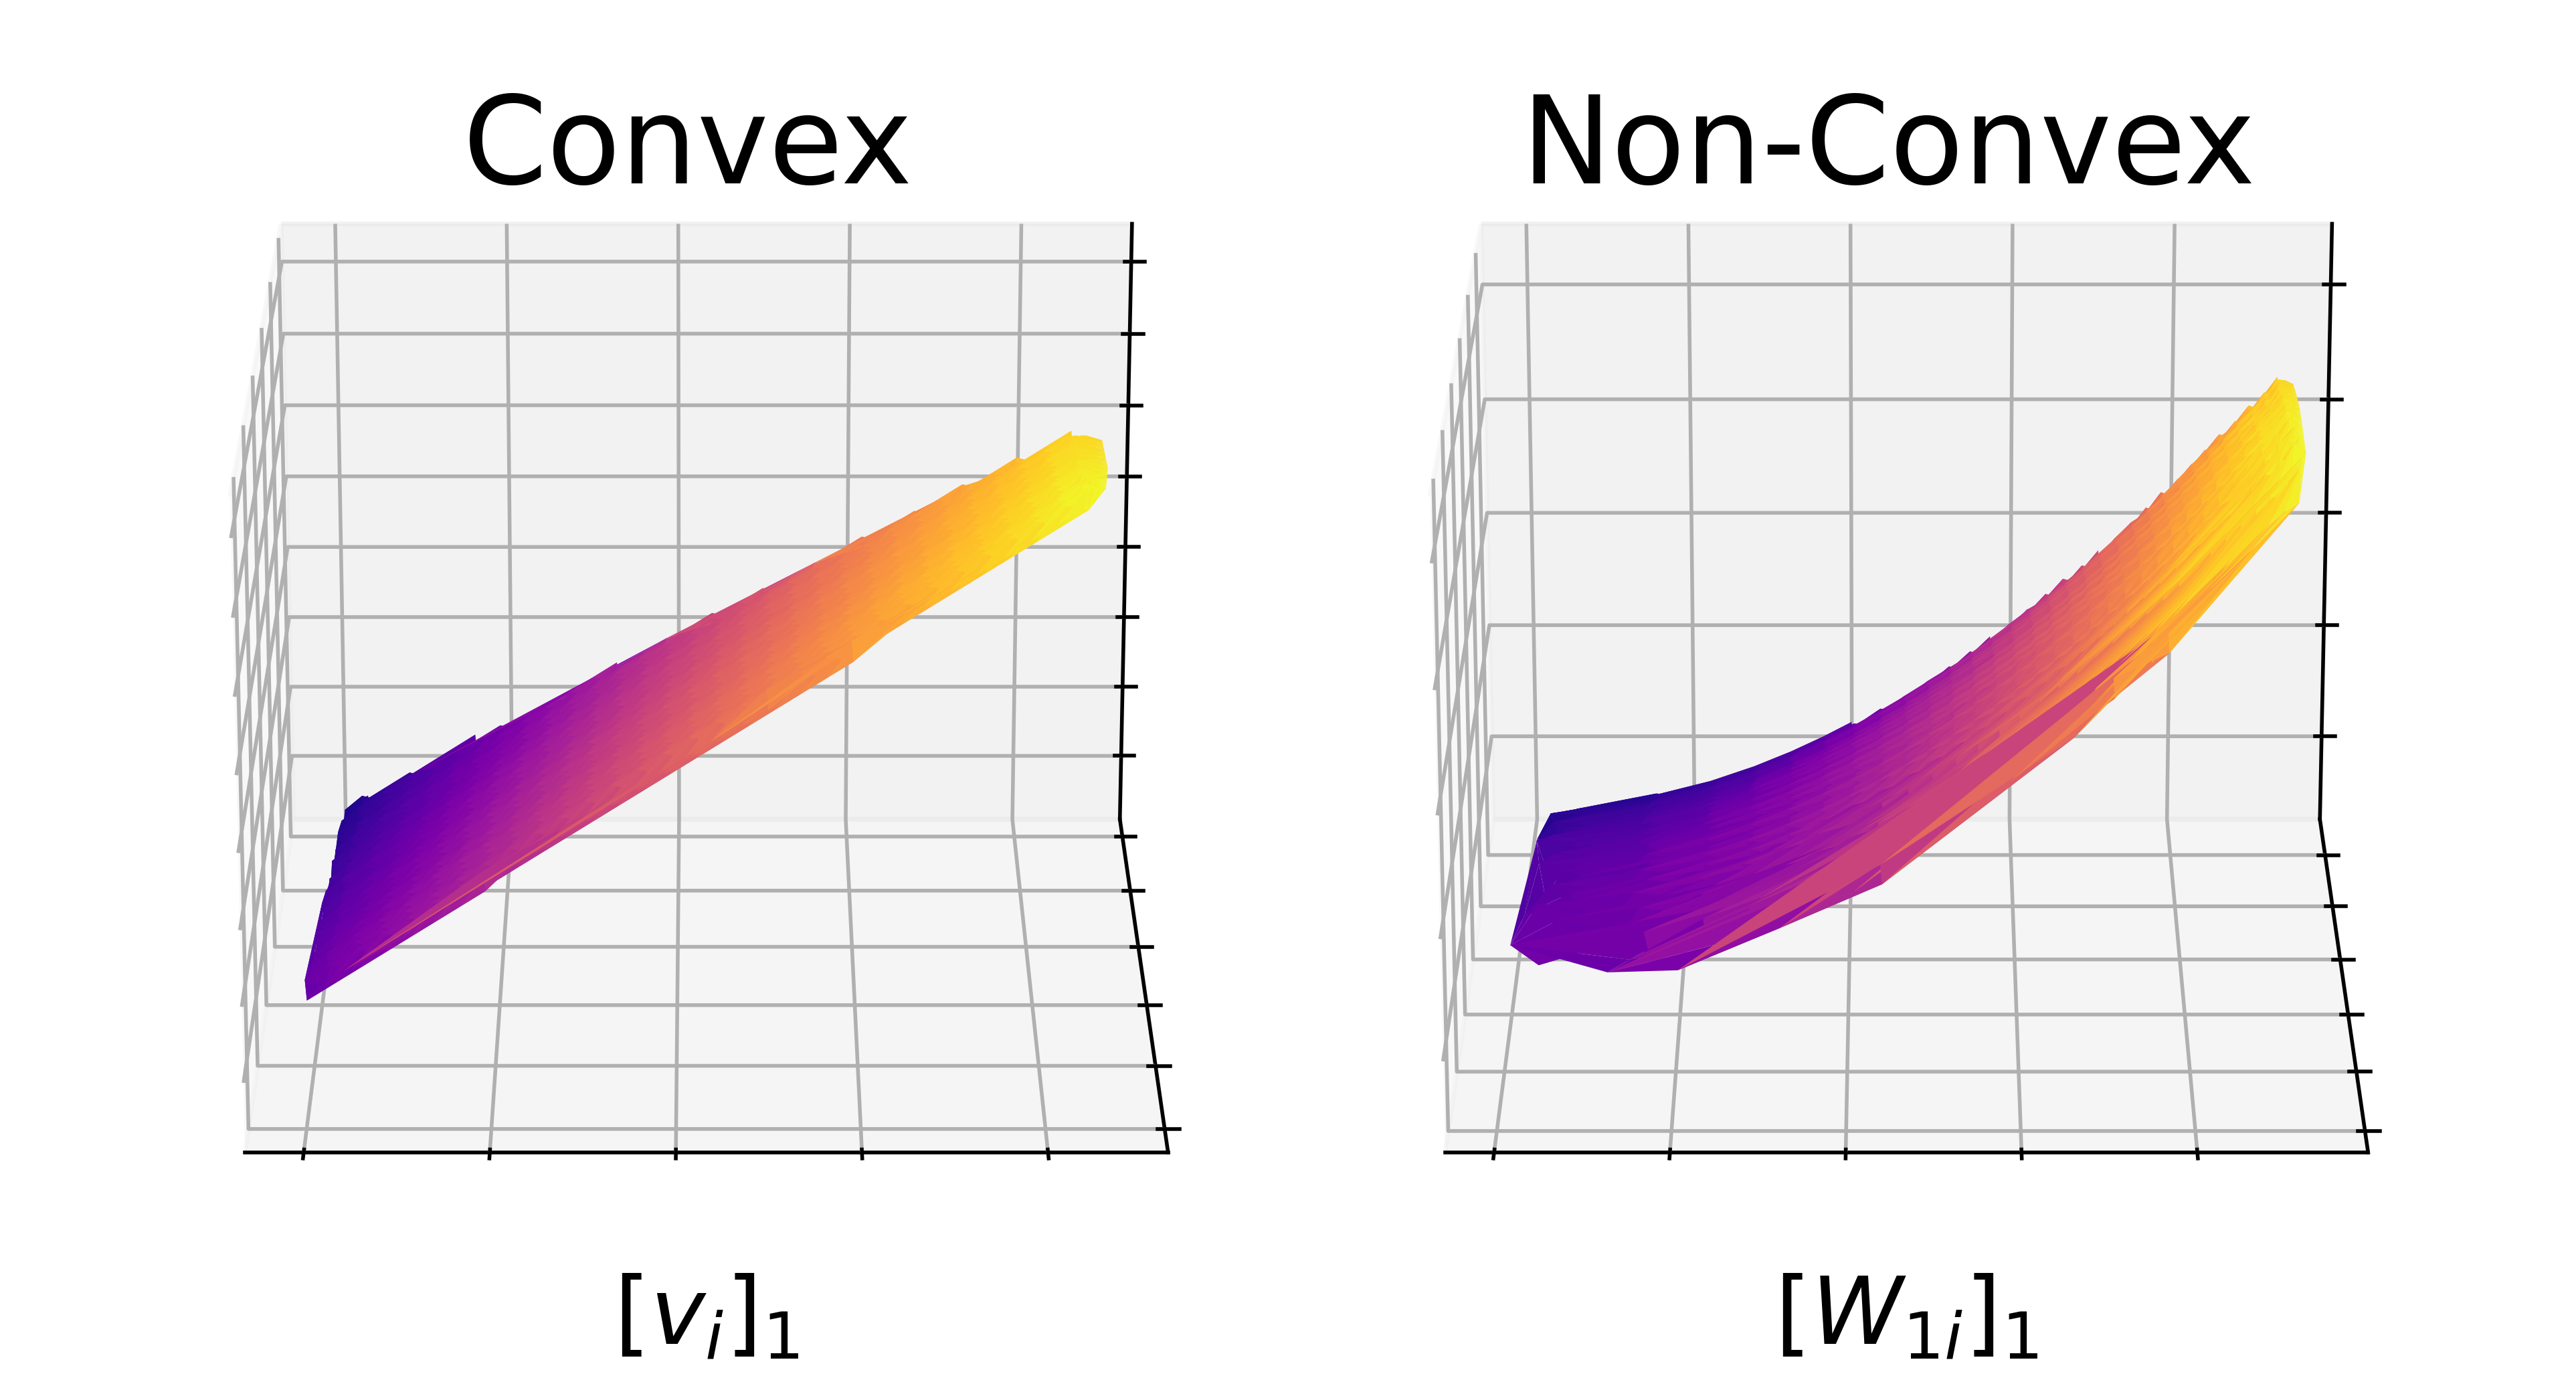
\includegraphics[width=.9\textwidth]{assets/solution_sets_vis_270.png}
					\caption{\textbf{Optimal set} for the first feature of three different
						neurons.}
					\vspace{-1em}
					\label{fig:solution-sets}
				\end{figure}

			\end{block}

			\begin{block}{Convex Reformulations: ReLU Networks}

				\begin{columns}[t]
					\begin{column}{0.62\textwidth}

						\large
						{\Large \red{Non-Convex Problem}:}
						\vspace{1em}
						{
							\Large
							\[
								\min_{\theta^1, \theta^2} \underbrace{\norm{\sum_{j=1}^m (X \theta^1_j)_+ \theta_j^2 - y}_2^2}_{\text{Squared Error}}
								+ \underbrace{\lambda \sum_{j=1}^m \norm{\theta^1_j}_2^2 + \norm{\theta^2_j}_2^2}_{\text{Weight Decay}},
							\]
						}
						where \( \rbr{x}_+ = \max\cbr{x, 0} \) is the ReLU activation.


						\vspace{2.5em}
						\hrule
						\vspace{2.5em}

						{\Large \blue{Convex Reformulation}}: {\normalsize \citep{pilanci2020convexnn}}
						\vspace{1em}
						{\Large
							\[
								\begin{aligned}
									\min_{u, h} & \norm{\sum_{j=1}^p D_j X (u_j - h_j) - y}_2^2 +
									\lambda \sum_{j=1}^p \norm{u_j}_2 + \norm{h_j}_2              \\
									            & \hspace{0.2em} \purple{\text{s.t. }
										u_j, h_j \in \calK_j := \cbr{w : (2D_j - I) X w \geq 0}},
								\end{aligned}
							\]
						}

						\vspace{1em}
						where \( D_j = \text{diag}[\mathbbm{1}(X g_j \geq 0)] \).

						\vspace{2.5em}
						\hrule
						\vspace{2.5em}


					\end{column}

					\begin{column}{0.55\textwidth}
						\vspace{-2em}

						\begin{figure}[]
							\centering
							\begin{tikzpicture}[scale=2.5,
	]
	\begin{axis}[width=0.4\linewidth, height=8cm,
			axis lines=none,  % don't print axis lines
			yticklabels={,,}, xticklabels={,,},
			ymin=0, ymax=8, y axis line style={-},
			xmin=0, xmax=15, x axis line style={-},
		]
		\node [Input] (input1) at (axis cs:3,2) {};
		\node [Input] (input2) at (axis cs:3,4) {};
		\node [Input] (input3) at (axis cs:3,6) {};

		\node [Hidden] (hidden1) at (axis cs:8,1) {};
		\node [Hidden] (hidden2) at (axis cs:8,3) {};
		\node [Hidden] (hidden3) at (axis cs:8,5) {};
		\node [Hidden] (hidden4) at (axis cs:8,7) {};

		\draw [->, style=arrow, draw=black] (input1) -- (hidden1);
		\draw [->, style=arrow, draw=black] (input2) -- (hidden1);
		\draw [->, style=arrow, draw=black] (input3) -- (hidden1);

		\draw [->, style=arrow, draw=black] (input1) -- (hidden2);
		\draw [->, style=arrow, draw=black] (input2) -- (hidden2);
		\draw [->, style=arrow, draw=black] (input3) -- (hidden2);

		\draw [->, style=arrow, draw=black] (input1) -- (hidden3);
		\draw [->, style=arrow, draw=black] (input2) -- (hidden3);
		\draw [->, style=arrow, draw=black] (input3) -- (hidden3);

		\draw [->, style=arrow, draw=red] (input1) -- (hidden4);
		\draw [->, style=arrow, draw=red] (input2) -- (hidden4);
		\draw [->, style=arrow, draw=red] (input3) -- (hidden4) node[pos=0.5,above] {$\theta^1_{j}$};

		\node [Output] (output) at (axis cs:13,4) {$\hat y$};

		\draw [->, style=arrow, draw=black] (hidden1) -- (output);
		\draw [->, style=arrow, draw=black] (hidden2) -- (output);
		\draw [->, style=arrow, draw=black] (hidden3) -- (output);
		\draw [->, style=arrow, draw=red] (hidden4) -- (output) node[pos=0.5,above] {$\theta^2_{j}$};
	\end{axis}

\end{tikzpicture}%

%\begin{tikzpicture}[scale=1,
%    ]
%    \begin{axis}[width=1.1\linewidth, height=5cm,
%            axis lines=none,  % don't print axis lines
%            yticklabels={,,}, xticklabels={,,},
%            ymin=-0.2, ymax=10.2, x axis line style={-},
%            xmin=-0.2, xmax=20.2, y axis line style={-},
%        ]

%        \filldraw[color=blue!60, fill=blue!5, line width=0.4mm](axis cs:0,5.8) rectangle (axis cs:20, 10);
%        \filldraw[color=red!60, fill=red!5, line width=0.4mm](axis cs:0,0) rectangle (axis cs:20, 4.2);

%        % non-convex models
%        \filldraw[line width=0.4mm, fill=white](axis cs:1,1) rectangle (axis cs:8, 3.2) node[pos=.5] {NC-GReLU};
%        \filldraw[line width=0.4mm, fill=white](axis cs:12,1) rectangle (axis cs:19, 3.2) node[pos=.5] {NC-ReLU};

%        % convex models
%        \filldraw[line width=0.4mm, fill=white](axis cs:1,6.8) rectangle (axis cs:8, 9) node[pos=.5] {C-GReLU};
%        \filldraw[line width=0.4mm, fill=white](axis cs:12,6.8) rectangle (axis cs:19, 9) node[pos=.5] {C-ReLU};

%        \draw [<->, solid, draw=black, line width = 0.6mm] (axis cs:4.5,3.2) -- (axis cs:4.5,6.8) node[right, pos=0.5] {\small Sol. Map};

%        \draw [<->, solid, draw=black, line width = 0.6mm] (axis cs:15.5,3.2) -- (axis cs:15.5,6.8)  node[right, pos=0.5] {\small Sol. Map};

%        \draw [<-, solid, draw=black, line width = 0.6mm] (axis cs:6,9) -- [bend left=15] (axis cs:14, 9);

%        \draw [->, solid, draw=orange, line width = 0.6mm] (axis cs:8,7.9) -- (axis cs:12,7.9);
%        \node[align=center] at (axis cs:10.1, 7.8) {\small Cone\\ \small Decomp.};
%    \end{axis}

%\end{tikzpicture}%


						\end{figure}

						\vspace{-3em}
						\begin{figure}[]
							\centering
							\begin{tikzpicture}[scale=2.5,
	]
	\begin{axis}[width=0.4\linewidth, height=8cm,
			axis lines=none,  % don't print axis lines
			yticklabels={,,}, xticklabels={,,},
			ymin=0, ymax=8, y axis line style={-},
			xmin=0, xmax=15, x axis line style={-},
		]
		\node [] (input1) at (axis cs:3,1) {$X$};
		\node [] (input2) at (axis cs:3,2.75) {$X$};
		\node [] (input3) at (axis cs:3,4.5) {$X$};

		\node [Splits] (hidden1) at (axis cs:9,1) {\scriptsize $D_3 X$};
		\node [Splits] (hidden2) at (axis cs:9,2.75) {\scriptsize $D_2 X$};
		\node [Splits] (hidden3) at (axis cs:9,4.5) {\scriptsize $D_1 X$};

		\draw [->, style=arrow, draw=black] (input1) -- (hidden1);

		\draw [->, style=arrow, draw=black] (input2) -- (hidden2);

		\draw [->, style=arrow, draw=red] (input3) -- (hidden3);

		\node [Output] (output) at (axis cs:13,2.75) {$\hat y$};

		\draw [->, style=arrow, draw=black] (hidden1) -- (output);
		\draw [->, style=arrow, draw=black] (hidden2) -- (output);
		\draw [->, style=arrow, draw=red] (hidden3) -- (output) node[pos=0.8,above] {$u_j$};

		\draw [draw=black, line width=0.3mm, dashed] (axis cs:4.65, 4.75) -- (axis cs:6.,6.6);
		\draw [draw=black, line width=0.3mm, dashed] (axis cs:6.5, 4.4) -- (axis cs:8.8,5.65);

		\node [draw=black, minimum size=0.2cm, shape=circle, solid, line width=0.5mm] (examine) at (axis cs:5.5,4.5) {};
		\node [draw=black, minimum size=1.4cm, shape=circle, solid, line width=0.5mm] (closeup) at (axis cs:7.5,6.2) {};

		\node [fill=white, draw=gray, line width=0.5mm, inner sep=0.07cm, shape=circle] at (axis cs:7.9,6.85) {};
		\node [fill=white, draw=gray, line width=0.5mm, inner sep=0.07cm, shape=circle] at (axis cs:7.15,6.9) {};
		\node [fill=white, draw=gray, line width=0.5mm, inner sep=0.07cm, shape=circle] at (axis cs:7.2,6.5) {};
		\node [fill=white, draw=gray, line width=0.5mm, inner sep=0.07cm, shape=circle] at (axis cs:6.3,6.25) {};

		\draw [draw=blue, dashed, line width=0.6mm] (axis cs:6.05,5.7) -- (axis cs:8.65,6.75);

		\node [fill=red, inner sep=0.08cm, shape=circle] at (axis cs:7.1,5.65) {};
		\node [fill=red, inner sep=0.08cm, shape=circle] at (axis cs:7.6,6.0) {};
		\node [fill=red, inner sep=0.08cm, shape=circle] at (axis cs:8.0,5.7) {};

	\end{axis}

\end{tikzpicture}%

%\begin{tikzpicture}[scale=1,
%    ]
%    \begin{axis}[width=1.1\linewidth, height=5cm,
%            axis lines=none,  % don't print axis lines
%            yticklabels={,,}, xticklabels={,,},
%            ymin=-0.2, ymax=10.2, x axis line style={-},
%            xmin=-0.2, xmax=20.2, y axis line style={-},
%        ]

%        \filldraw[color=blue!60, fill=blue!5, line width=0.4mm](axis cs:0,5.8) rectangle (axis cs:20, 10);
%        \filldraw[color=red!60, fill=red!5, line width=0.4mm](axis cs:0,0) rectangle (axis cs:20, 4.2);

%        % non-convex models
%        \filldraw[line width=0.4mm, fill=white](axis cs:1,1) rectangle (axis cs:8, 3.2) node[pos=.5] {NC-GReLU};
%        \filldraw[line width=0.4mm, fill=white](axis cs:12,1) rectangle (axis cs:19, 3.2) node[pos=.5] {NC-ReLU};

%        % convex models
%        \filldraw[line width=0.4mm, fill=white](axis cs:1,6.8) rectangle (axis cs:8, 9) node[pos=.5] {C-GReLU};
%        \filldraw[line width=0.4mm, fill=white](axis cs:12,6.8) rectangle (axis cs:19, 9) node[pos=.5] {C-ReLU};

%        \draw [<->, solid, draw=black, line width = 0.6mm] (axis cs:4.5,3.2) -- (axis cs:4.5,6.8) node[right, pos=0.5] {\small Sol. Map};

%        \draw [<->, solid, draw=black, line width = 0.6mm] (axis cs:15.5,3.2) -- (axis cs:15.5,6.8)  node[right, pos=0.5] {\small Sol. Map};

%        \draw [<-, solid, draw=black, line width = 0.6mm] (axis cs:6,9) -- [bend left=15] (axis cs:14, 9);

%        \draw [->, solid, draw=orange, line width = 0.6mm] (axis cs:8,7.9) -- (axis cs:12,7.9);
%        \node[align=center] at (axis cs:10.1, 7.8) {\small Cone\\ \small Decomp.};
%    \end{axis}

%\end{tikzpicture}%


						\end{figure}

					\end{column}
				\end{columns}

				\large
				\vspace{-1em}
				{\Large \blue{Equivalence}}:
				\vspace{0.25em}

				\begin{itemize}
					\item If \( m \geq m^* \), where \( m^* \leq n \),
					      then both programs have the same optimal value.

					\item The convex and non-convex solutions are related by a
					      \textbf{solution mapping}.
				\end{itemize}


			\end{block}

		\end{column}

		\separatorcolumn

		\begin{column}{\colwidth}

			\vspace{-1.5em}
			\begin{block}{Proof Strategy}
				\large

				{\Large
					\blue{Approach}: We use convex reformulations as an analytical tool!
				}
				\begin{enumerate}
					\item Re-write convex reformulation as a \textbf{constrained group lasso} (CGL) problem,
					      {\Large
							      \begin{equation*}\label{eq:constrained-gl}
								      \begin{aligned}
									      p^*(\lambda) = \min_{w} \,
									       & \half \norm{Z w - y}_2^2 + \lambda \sum_{\bi \in \calB} \norm{\wi}_2                  \\
									       & \quad \text{s.t.} \quad \purple{\Ki^\top \wi \leq 0}  \text{ for all } \bi \in \calB.
								      \end{aligned}
							      \end{equation*}
						      }
					\item Derive optimal set for CGL using the \textbf{KKT conditions}: if \( \wi \neq 0 \),
					      {
							      \Large
							      \begin{equation*}\label{eq:kkt-cgl}
								      \underbrace{\red{Z_{\bi}^\top (y - Z w) - \Ki \ri}}_{\vi} = \lambda \frac{\wi}{\norm{\wi}_2}
							      \end{equation*}
						      }

					\item Obtain ReLU optimal set using the \textbf{solution mapping}: for \( s_i \in \cbr{+1, -1} \),

					      { \Large
							      \begin{equation*}\label{eq:convex-to-relu}
								      \theta_{i}^1 = \wi^*/ \sqrt{\norm{\wi^*}}, \quad \theta_{i}^2 = s_i \cdot \sqrt{\norm{\wi^*}}
							      \end{equation*}
						      }

				\end{enumerate}

			\end{block}

			\vspace{-1em}
			\begin{block}{The ReLU Optimal Set}

				\large

				Define the set of blocks supported by \emph{a solution} to the convex reformulation:
				\[
					\calS_\lambda = \cbr{\bi \in \calB : \exists w \in \solfn(\lambda), \wi \neq 0},
				\]
				and let \( Z w^* = \hat y \) be the (unique) optimal model fit.

				\vspace{1em}

				\begin{beamercolorbox}[wd=\textwidth,sep=1em]{result}

					\textbf{Corollary 4.1} (informal):
					Suppose \( m \geq m^* \) and \( \lambda > 0 \).
					Then the set of optimal two-layer ReLU MLPs is,

					\begin{equation*}\label{eq:relu-sol-fn}
						\Large
						\begin{aligned}
							\calO_\lambda  = \,
							\big\{
							(W_1,  w_2) : &
							\, f_{\theta^1, \theta^2}(Z)  =  \hat y,                                                        \\
							              & \theta^1_{i} = \rbr{\frac{\alpha_{i}}{\lambda}}^{\frac{1}{2}} v_i,
							\theta_{i}^2 = \rbr{\alpha_i \lambda}^{\frac{1}{2}},                                            \\
							              & \alpha_i \geq 0, \, i \in [2p] \setminus \calS_\lambda \Rightarrow \alpha_i = 0
							\big\},
						\end{aligned}
					\end{equation*}
				\end{beamercolorbox}

				\textbf{Interpretation}: optimal neurons are scalings of the correlation vector \( \red{\vi} \)
				on the \blue{manifold of optimal predictors}.

			\end{block}
			\vspace{-1em}
			\begin{block}{Conditions for Uniqueness}
				\large

				{ \Large
					\red{Q}: When are optimal networks unique up to permutations/splits?

					\vspace{0.5em}

					\blue{A}: When the convex reformulation has a unique solution!
				}
				\vspace{0.5em}

				\begin{beamercolorbox}[wd=\textwidth,sep=1em]{result}
					\textbf{Proposition 4.3} (informal):
					Suppose \( m \geq m^* \) and \( \lambda > 0 \).
					If there does not exist \( \alpha \neq 0 \) such that
					\[
						\Large
						\sum_{i\in \calS_\lambda } \alpha_i (X \theta^1_{i})_+ = 0,
					\]
					then the non-convex solution is permutation/splitting
					unique (p-unique).
				\end{beamercolorbox}

				\textbf{Continuity}: p-uniqueness on a neighbourhood \( \calN \)
				implies continuity of at least one regularization path
				\( \lambda \mapsto (\theta^1(\lambda), \theta^2(\lambda)) \) on \( \calN \).

			\end{block}
		\end{column}

		\separatorcolumn

		\begin{column}{\colwidth}
			\vspace{-1.5em}
			\begin{block}{Optimal Pruning}
				\large
				\textbf{Definition}: a ReLU network is \blue{minimal}
				if there does not exist an optimal network with strictly
				fewer non-zero neurons.

				\vspace{0.5em}

				\begin{beamercolorbox}[wd=\textwidth,sep=1em]{result}
					\textbf{Proposition 3.6} (informal):
					Let
					\( m \geq m^* \) and \( \lambda > 0 \).
					A model is minimal if and only if the non-zero
					activations \( (X \theta^1_{i})_+ \) are linearly independent.
				\end{beamercolorbox}

				\vspace{0.5em}

				\begin{algorithm}[H]
	\Large
	\caption{\large Optimal Pruning}
	\label{alg:pruning-solutions}
	\begin{algorithmic}
		\STATE {\large {\bfseries Input:} data matrix \( Z \), solution \( w^0 \).}
		\WHILE {\( \exists \beta \neq 0 \) s.t. \( \sum_{\bi \in \act(w^k)} \beta_\bi Z_{\bi} \wi^k = 0 \)}
		\STATE \( \bi^k \gets \argmax_{\bi} \cbr{|\beta_\bi| : \bi \in \act(w^k)}  \)
		\STATE \( t^k \gets 1/|\beta_{\bi^k}| \)
		\STATE \( \w^{k+1} \gets \w^k (1 - t^k \beta_\bi) \)
		\ENDWHILE
		\STATE {\bfseries Output:} final weights \( \w^k \)
	\end{algorithmic}
\end{algorithm}




				\begin{beamercolorbox}[wd=\textwidth,sep=1em]{result}
					\textbf{Proposition} (informal):
					Algorithm 1 computes an optimal and minimal ReLU network with
					\( m^* \leq n \) non-zero neurons in
					\( O(n^3 m + nd) \) time.
				\end{beamercolorbox}

				\textbf{Direct Pruning}: We give equivalent algorithm
				for non-convex params.


			\end{block}
			\vspace{-1em}
			\begin{block}{Experiments}
				\large

				%{\Large \blue{Goal}: highlight practical consequences of our theory.}

				\begin{figure}[]
					\centering
					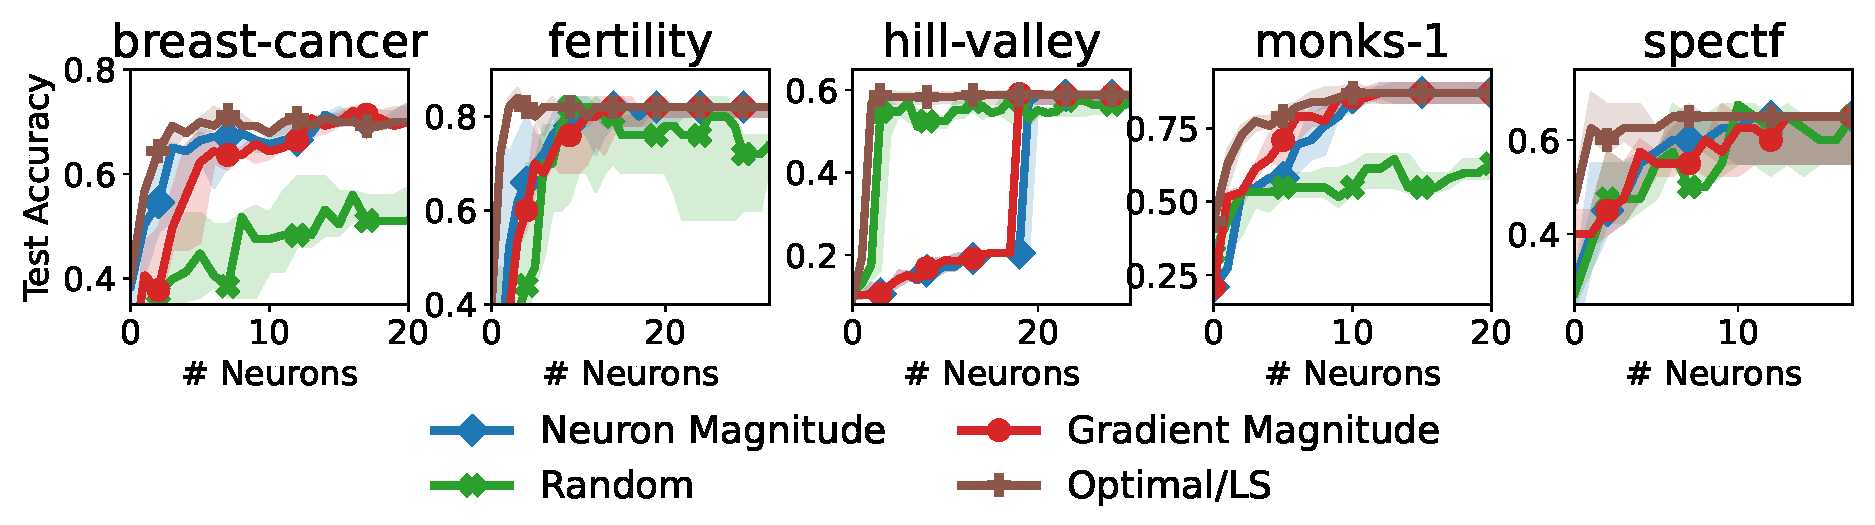
\includegraphics[width=\textwidth]{assets/uci_pruning_acc.pdf}
					\label{fig:purning}
					\vspace{-2em}
					\caption{Test accuracy for theory-inspired pruning (Optimal/LS) and baseline methods.}
				\end{figure}
				\vspace{-0.5em}
				\begin{itemize}
					\item We consider pruning neurons on several UCI
					      classification datasets.
					\item Our approach \blue{dominates} every baseline considered.
				\end{itemize}

				\vspace{-0.5em}
				\begin{table}[t]
	\centering
	\label{table:tuning-small}
	\begin{tabular}{lccccc} \toprule
		\textbf{Dataset} & \textbf{Min L$_2$} & \textbf{EP} & \textbf{V-MSE} & \textbf{T-MSE} & \textbf{Max Diff.} \\
		\midrule
		mammogr.         & 0.77               & 0.77        & 0.57           & 0.78           & \textbf{0.21}      \\
		horse-colic      & 0.75               & 0.59        & 0.74           & 0.85           & \textbf{0.26}      \\
		ilpd-indian      & 0.59               & 0.59        & 0.53           & 0.72           & \textbf{0.19}      \\
		parkinsons       & 0.74               & 0.74        & 0.65           & 0.88           & \textbf{0.23}      \\
		pima             & 0.68               & 0.68        & 0.68           & 0.87           & \textbf{0.2}       \\
		\bottomrule
	\end{tabular}
\end{table}

				\begin{itemize}
					\item We tune ReLU networks by direct optimization over the optimal set.
					\item Same training performance, but test accuracy differs by over \red{20 points}!
				\end{itemize}

			\end{block}
			\vspace{-1em}

			\begin{block}{References}

				\footnotesize{
					\bibliography{
						bib/monographs.bib,
						bib/gradient_methods.bib,
						bib/lower_bounds.bib,
						bib/assumptions.bib,
						bib/interpolation.bib,
						bib/step_sizes.bib,
						bib/datasets.bib,
						bib/general_refs.bib}
				}
				\bibliographystyle{icml2023}

			\end{block}

		\end{column}

		\separatorcolumn
	\end{columns}
\end{frame}

\end{document}
